\Def Назовём \textit{предельной точкой} такое $\alpha$, что в любой окрестности $\alpha$ существует $\alpha'$, для которого не выполнен закон нуля или единицы.

Докажем, что в языке $\mathcal{L}^3$ предельные точки существуют в любой левой полуокрестности единицы: 
$\forall \varepsilon > 0 ~ \exists \alpha \in (1 - \varepsilon, 1)$.

Рассмотрим граф, состоящий из $k+2$ треугольников, соединённых простыми путями.
Причём, расстояние (в рёбрах) между вторым и третьим треугольниками, третьим и четвёртым и т. д., одинаково.
Обозначим это расстояние $m$, а расстояние между первым и вторым треугольником - $s$.

\begin{figure}[h]
    \centering
  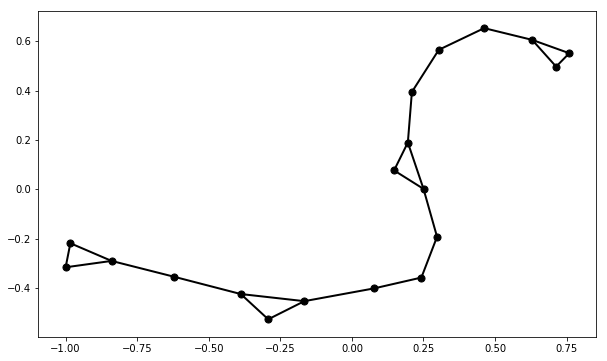
\includegraphics[scale=0.4]{picrel/index.png}
  \caption{Граф с $k = 2$, $s = 2$ и $m = 4$}
  \label{fig:chain1}
\end{figure}

Плотность такого графа равна 
$$\rho_{H_{ksm}} = \dfrac{6+s + (3+m)k}{5+s + (2+m)k}$$
и при увеличении $k$ стремится к $\rho_\infty = \dfrac{3+m}{2+m}$.

Граф с $k=0$ состоит из двух треугольников и имеет вид гантели.

Т.к. 
$sign\left(\dfrac{\partial\rho_{H_{ksm}}}{\partial k}\right) = sign(3+s-m)$,
то при $m < 3 + s$ плотность графа растёт при увеличении  $k$ и, как нетрудно убедиться, при этом выполнено равенство
$\rho_{H_{ksm}} = \rho^{max}_{H_{ksm}}$.
Будем считать $m = s+2$, т.к. при таком соотношении длины гантели и длины добавочных звеньев
граф получается оптимальным с точки зрения плотности, что пригодится в дальнейшем.

Таким образом, для доказательства утверждения достаточно предъявить для каждого такого графа формулу из  $\mathcal{L}^3$, выражающую его существование.

Вместо 
$\exists x \exists y \exists z ~ x \sim y \wedge y \sim z \wedge x \sim z$
будем писать 
$\exists x~\triangle_{xyz}$

Формула, выражающая существование гантели, имеет вид:
\def\gantelRightPart {
&\wedge \exists x ~ 
    \left[ x \sim z \wedge x \neq y \wedge x \nsim y  \right] \\
&\wedge \exists y ~
    \left[ y \sim x \wedge y \neq z \wedge y \nsim z \right] \\
&\wedge \exists z ~
    \left[ z \sim y \wedge z \neq x \wedge z \nsim x  \right] \\
&\wedge ~ \qquad \qquad \cdots \\
&\wedge \exists x ~ 
    x \sim z \wedge x \sim y
}

\begin{equation}
\label{f:gantel}
\begin{split}
\exists x~\triangle_{xyz} \gantelRightPart,
\end{split}
\end{equation}
где количество выражений в квадратных скобках равно числу вершин между треугольниками минус 2

Формула $\varphi_{ksm} $, выражающая существование графа $H_{ksm}$, выглядит аналогично, только часть формулы (\ref{f:gantel}), следующая за 
$\exists x~\triangle_{xyz}$,
содержит $s-1$ выражение в квадратных скобках и повторяется ещё $k$ раз, и каждая из повторяющихся частей содержит $m-1 $ выражение в квадратных скобках.
% \begin{equation}
% \label{f:phiKsm}
% \left. 
%     \begin{split}
%         \exists x~\triangle_{xyz} 
%         \gantelRightPart
% \right\}
% \left. 
%     \left. \gantelRightPart \right\}
%     \left. \gantelRightPart \right\}
% \right\}
% \end{equation}

% \[
% \begin{split}
% \left.
% a = b \\
% c = d
% \right\}
% \end{split}
% \]

Конечно, вообще, существование в $G(n, n^{-\alpha})$ подграфа $H_{ksm}$ не является необходимым для того, чтобы формула $\varphi_{ksm}$ была верна.
Однако, оно становится необходимым при $\alpha = 1/\rho_{H_{ksm}}$ и $m = s+2$. 
Действительно, покажем, что любой другой граф $\tilde H_{ksm}$, для которого выполнено $\varphi_{ksm}$, имеет максимальную плотность большую, чем $\rho_{H_{ksm}}$.

\begin{Lem} 
\label{lem:min_ro_Hksm}
Граф $H_{ksm}$ имеет минимальную $\rho^{max}$ среди всех графов, для которых выполнено $\varphi_{ksm}$
\end{Lem}

\begin{proof}
В графе $H_{ksm}$ каждой переменной формулы $\varphi_{ksm}$ соответствует отдельная вершина.
Любой другой граф $\tilde H_{ksm}$ либо получается путём добавления рёбер в $H_{ksm}$ (в этом случае увеличение плотности очевидно), либо имеет вершину, которой соответствует более одной переменной.
Далее будем рассматривать только второй случай.
Пусть в звене под номером $k'$ (номер $0$ соответствует гантели), впервые произошло повторное ``использование'' вершины. 

Более строго $k'$ можно определить так:

Равенство
$\varphi_{ksm}(\tilde H_{ksm}) = 1$
означает, что существует такая сюръекция из множества вершин графа во множество переменных формулы, что если в формулу вместо переменных подставить соответствующие вершины, получится верное утверждение.
Зафиксируем это соответствие.
Для каждого $k' < k$ определим $\tilde H'_{k'sm}$ как подграф $\tilde H_{ksm}$, индуцированный на множество вершин, соответствующее переменным, входящим в подформулу формулы $\varphi_{ksm}$, совпадающую с $\varphi_{k'sm}$.
Пусть теперь $k' \in $ такое, что в $\tilde H_{k'sm}$ есть вершина, которой соответствуют две переменные, а (если $k' \neq 0$) в $~\tilde H_{k'-1,sm}$ таких вершин нет.\\
$e:= e(H_{k'sm})$ , $v:= v(H_{k'sm})$\\
$\tilde e:= e(\tilde H_{k'sm})$ , $\tilde v:= v(\tilde H_{k'sm})$\\
Есть три возможности:
\begin{enumerate}
\item 
Последняя вершина в звене уже была использована - та, которая сразу добавляет два ребра
\begin{enumerate}
\item 
повторно использована только она: $\tilde \rho^{max} \geq \dfrac{e}{v-1}$ \\
В этом случае число вершин в $\tilde H_{k'sm}$ равно $v-1$, а число рёбер не меньше $e$. Действительно, в рассматриваемом случае (по определению) $\tilde H_{k'sm}$ содержит все рёбра $H_{k'sm}$, кроме, быть может, двух рёбер, инцидентных последней вершине, которые могут уже присутствовать в $H_{k'sm}$
Однако, легко видеть, что это невозможно (см. Рис. \ref{fig:only last reused}).
\begin{figure}
  \centering
  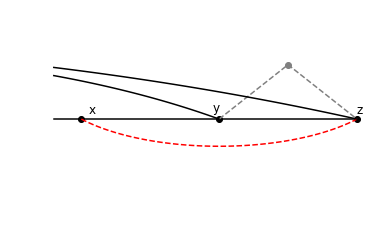
\includegraphics[scale=0.5]{picrel/only_last_reused.png}
  \caption{Только последняя вершина использована повторно. Черным обозначены вершины и рёбра $\tilde H_{k'sm}$, серым вершины и рёбра  $H_{k'sm}$, красным пунктиром - рёбра, запрещённые формулой  }
  \label{fig:only last reused}
\end{figure}
\item
она и какая-то до неё: $\tilde \rho^{max} \geq \dfrac{e-2}{v-2}$ \\
\begin{figure}
  \centering
  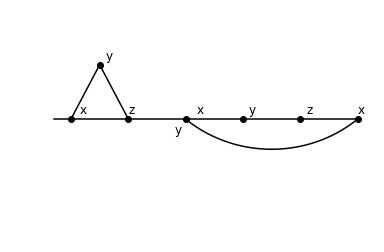
\includegraphics[scale=0.5]{picrel/reuse_intermediate.png}
  \caption{Повторное использование промежуточной вершины}
  \label{fig:reuse intermediate}
\end{figure}
\label{enum:reuse intermediate}
Посмотрим на первую повторно использованную вершину.
Т.к. формула запрещает совпадать вершинам, соответствующим разным переменным, для её соединения с предыдущими вершинами необходимо добавить ребро, которого нет в графе $H_{k'sm}$. 
С каждой новой секцией в $H_{k'sm}$ добавляется $3+m$ рёбер  и $2+m$ вершин.
Однако, проведя дополнительное ребро к уже имеющейся вершине, мы уже добавили на одно ребро больше, чем вершин, поэтому имеем рёбер $ e - (3+m) + (\nu+1) = e - (m-\nu) $, вершин $v - (2+m) + \nu = v - (m-\nu)$, где $\nu$ - число вершин, уже добавленных в последней, ,,секции'' $\tilde H_{k'sm}$.
Поскольку $\tilde H_{k'sm}$ связен, при добавлении новой вершины добавляется и как минимум одно ребро.
В рассматриваемом случае $\tilde v \leq v-2$, поэтому $\tilde \rho^{max} \geq \frac{e-2}{v-2}$ 
\end{enumerate}
\item
Последняя вершина ещё не была использована:
$\tilde \rho^{max} \geq \dfrac{e}{v-1}$\\
Случай похож на \ref{enum:reuse intermediate}, но теперь $\tilde v \leq v-1$ и последняя вершина добавляет 2 ребра
\end{enumerate}

Итого 
$\tilde \rho^{max} \geq \dfrac{e-2}{v-2} = \dfrac{4+s +(3+m)k'}{3+s + (2+m)k'}$. 

Используя $m=s+2$, получаем $\tilde \rho - \rho_\infty = \dfrac{1}{((2+m)(k+1)-1)(m+2)}$, следовательно
$\tilde \rho^{max} > \rho_\infty > \rho_{H_{ksm}} $.
\end{proof}

Из теоремы \ref{th:ruchinski} и леммы \ref{lem:min_ro_Hksm} следует следующий результат

\begin{theorem}
 Закон нуля или единицы для языка $\LL^3$ нарушается в точках $\alpha = \frac{m+3 + (2+m)k}{m+4 + (3+m)k}$, $m \geq 3$, $k \geq 0$.
В языке $\LL^3$ есть предельные точки в любой левой полуокрестности единицы.
\end{theorem}